\documentclass[12pt,a4paper,oneside]{book}
\usepackage[utf8]{vietnam}
\usepackage[utf8]{inputenc}
\usepackage[top=3cm, bottom=3.5cm, left=3.5cm, right=2.0cm]{geometry}  % căn lề theo quy chuẩn KLTN
\usepackage{mathptmx}   %time new roman
\usepackage{xcolor}
\usepackage{titlesec}
\usepackage{mathtools}
\DeclarePairedDelimiter{\abs}{\lvert}{\rvert}
\usepackage{graphicx}
\usepackage[export]{adjustbox}
\usepackage{mdframed}
\usepackage{amsmath}    
\usepackage{fancybox} 
\usepackage{fancyhdr}
\usepackage{setspace}
\usepackage{enumitem}
\usepackage{tabularx,array}
\usepackage[unicode]{hyperref}  %đánh chỉ mục
\usepackage{indentfirst}    %thụt đầu dòng đoạn đầu tiên
\usepackage{lipsum} %dummy text
\usepackage{sectsty}
\usepackage{multirow}
\usepackage{hhline}
\usepackage{amsfonts}
\usepackage{amssymb}

\chapternumberfont{\LARGE} 
\chaptertitlefont{\centering \huge}


\makeatletter
\renewcommand\section{\leftskip 0pt\@startsection {section}{1}{\z@}%
                                   {-3.5ex \@plus -1ex \@minus -.2ex}%
                                   {2.3ex \@plus.2ex}%
                                   {\normalfont\Large\bfseries}}
\renewcommand\subsection{\leftskip 25pt\@startsection{subsection}{2}{\z@}%
                                     {-3.25ex\@plus -1ex \@minus -.2ex}%
                                     {1.5ex \@plus .2ex}%
                                     {\normalfont\large\bfseries\leftskip 6ex}}
\renewcommand\subsubsection{\leftskip 50pt\@startsection{subsubsection}{2}{\z@}%
                                     {-3.25ex\@plus -1ex \@minus -.2ex}%
                                     {1.5ex \@plus .2ex}%
                                     {\normalfont\large\bfseries\leftskip 10ex}}
\makeatother

\setcounter{secnumdepth}{5}
\setcounter{tocdepth}{5}
\pagenumbering{gobble}
\pagestyle{fancy}
\fancyhf{}
\cfoot{\thepage}                    %   đánh số trang
\renewcommand{\headrulewidth}{0pt}
\renewcommand{\footrulewidth}{1,2pt}  
\allowdisplaybreaks 
\begin{document} 

%-	Bìa cứng - màu xanh dương, chữ mạ vàng (xem mẫu đính kèm)
%-	Trang tên (tờ lót): chất liệu giấy, nội dung giống như bìa LV
%-	Ở gáy LV: in nhan đề LV (có thể in tóm tắt nếu nhan đề quá dài), size 15 – 17
%-	Phiếu Nhiệm vụ LV, chấm điểm Hướng dẫn & Phản biện (đã ký): nhận từ GVHD & GVPB sau khi bảo vệ (theo lịch hẹn).
%-	Lời cam đoan
%-	Lời cảm ơn/ Lời ngỏ
%-	Tóm tắt LV
%-	Mục lục
%-	Danh mục, bảng biểu, hình ảnh, ... (nếu có)
%-	Nội dung LV
%-	Danh mục TL tham khảo
%-	Phụ lục (nếu có)

\fontsize{13pt}{18pt}\selectfont   % cỡ chữ 13, cỡ dòng 18
\setlength{\baselineskip}{18truept}


\begin{titlepage}
\begin{center}
{\large\bf ĐẠI HỌC QUỐC GIA TP. HỒ CHÍ MINH} \\
{\large\bf TRƯỜNG ĐẠI HỌC CÔNG NGHỆ THÔNG TIN}\\
{\Large\bf KHOA MẠNG MÁY TÍNH VÀ TRUYỀN THÔNG}\\[0.25cm]
\vskip 2.5cm
{\bf\large NGUYỄN ĐÌNH THANH - 16521119}\\
{\bf\large TRƯƠNG THỊ THANH NHÃ - 16520861}
\vskip 2.5cm
{\bf\Large KHÓA LUẬN TỐT NGHIỆP}\\[0.5cm]
{\LARGE\textbf{PHÁT TRIỂN ỨNG DỤNG NHẬN DIỆN ĐỐM LỬA DỰA TRÊN VIỆC ÁP DỤNG TRÍ THÔNG MINH NHÂN TẠO TẠI MẠNG CÂN BIÊN}}\\[0.5cm]
{\bf\Large\color{red} DEVELOPMENT OF FIRE DETECTION APPLICATION BASED ON APPLYING ARTIFICIAL INTELLIGENCE AT THE EDGE NETWORK}\\
\vskip 2.0cm
{\bf\large KỸ SƯ NGÀNH AN TOÀN THÔNG TIN}
\vfill
{\bf TP. HỒ CHÍ MINH, 2020}
\end{center}
\end{titlepage}

\thisfancypage{\setlength{\fboxsep}{10pt}\fbox}{}  %vẽ hộp vuông

\begin{titlepage}
\begin{center}
{\large\bf ĐẠI HỌC QUỐC GIA TP. HỒ CHÍ MINH} \\
{\large\bf TRƯỜNG ĐẠI HỌC CÔNG NGHỆ THÔNG TIN}\\
{\Large\bf KHOA MẠNG MÁY TÍNH VÀ TRUYỀN THÔNG}\\[0.25cm]
\vskip 2.5cm
{\bf\large NGUYỄN ĐÌNH THANH - 16521119}\\
{\bf\large TRƯƠNG THỊ THANH NHÃ - 16520861}
\vskip 2.5cm
{\bf\Large KHÓA LUẬN TỐT NGHIỆP}\\[0.5cm]
{\LARGE\textbf{PHÁT TRIỂN ỨNG DỤNG NHẬN DIỆN ĐỐM LỬA DỰA TRÊN VIỆC ÁP DỤNG TRÍ THÔNG MINH NHÂN TẠO TẠI MẠNG CÂN BIÊN}}\\[0.5cm]
{\bf\Large\color{red} DEVELOPMENT OF FIRE DETECTION APPLICATION BASED ON APPLYING ARTIFICIAL INTELLIGENCE AT THE EDGE NETWORK}\\
\vskip 2.0cm
{\bf\large KỸ SƯ NGÀNH AN TOÀN THÔNG TIN}
\vskip 1.0cm
{\bf\large GIẢNG VIÊN HƯỚNG DẪN}\\[0.20cm]
{\bf\large PGS.TS. LÊ TRUNG QUÂN}
\vfill
{\bf TP. HỒ CHÍ MINH, 2020}
\end{center}
\end{titlepage}


\chapter*{\centering Lời cảm ơn}
Đầu tiên, nhóm xin gửi lời cảm ơn sâu sắc đến toàn thể các thầy cô trong Trường Đại học Công Nghệ Thông Tin nói chung, và các thầy cô trong Khoa Mạng máy tính và Truyền thông nói riêng. Nhờ những kiến thức quý giá mà thầy cô đã truyền đạt, cũng như việc hỗ trợ tận tình trong suốt khoảng thời gian thực hiện, nhóm đã hoàn thành được khoá luận theo đúng tiến độ và đạt được các kết quả như mong đợi.

Nhóm xin đặc biệt cảm ơn PGS.TS Lê Trung Quân, người đã truyền cảm hứng, tận tình hướng dẫn và hỗ trợ từ kiến thức đến trang thiết bị cần thiết, cũng như tạo môi trường cho nhóm có cơ hội học hỏi từ các anh chị có kinh nghiệm đi trước. 

Bên cạnh đó, nhóm không quên bày tỏ lòng tri ân đến gia đình, người thân, các bạn trong lớp ANTN2016 và các anh chị trong khoa Mạng máy tính và Truyền thông, là những người đã đồng hành và giúp đỡ nhóm rất nhiều trong suốt quá trình tìm hiểu và hoàn thành khóa luận này.

Mặc dù nhóm đã nỗ lực rất nhiều để hoàn thiện khóa luận, song khó có thể tránh khỏi những thiếu sót và hạn chế. Kính mong nhận được sự thông cảm và ý kiến đóng góp từ quý thầy cô và các bạn.
\vspace{1cm}
\begin{flushright}\textit{Tp.Hồ Chí Minh, ngày 19 tháng 05 năm 2020}\end{flushright}
\vspace{-1.1cm}
\begin{center}\hspace{8cm}Nhóm tác giả\end{center}


\tableofcontents	                        % mục lục
%\listofsymbols
\let\origaddvspace\addvspace
\renewcommand{\addvspace}[1]{}
\listoffigures                              % hình ảnh
\renewcommand{\addvspace}[1]{\origaddvspace{#1}}
\listoftables                               % bảng
%\listofalgorithms

\linespread{1.25}   %dãn dòng 1.5 lines : 1.2 x 1.25  theo fomat
\setlength{\parskip}{1em} %giãn đoạn auto

\chapter*{\centering Tóm tắt luận văn}
\pagenumbering{arabic}                      %bắt đầu đánh số
\addcontentsline{toc}{chapter}{{\bf  Tóm tắt luận văn}\rm}
Đề tài luận văn này tập trung vào việc giải quyết....
\chapter*{\centering Mở đầu}
\addcontentsline{toc}{chapter}{{\bf  Mở đầu}\rm}

\section{Mở đầu}
Dựa trên những công việc mà nhóm thực hiện trong khóa luận cũng như cấu tạo của mô hình đề tài, cấu trúc của luận văn được tổ chức thành các phần tương ứng như sau:
\begin{itemize}
    \item {\bf Chương 1}: Tổng quan một số công trình nghiên cứu liên quan
    \item {\bf Chương 2}: Cung cấp cơ sở lý thuyết và các kiến thức nền tảng
    \item {\bf Chương 3}: Trình bày chi tiết mô hình đề xuất và phương hướng tiếp cận
\end{itemize}

\subsection{Khối lượng công việc}
Dựa trên những công việc mà nhóm thực hiện trong khóa luận cũng như cấu tạo của mô hình đề tài, cấu trúc của luận văn được tổ chức thành các phần tương ứng như sau:
\begin{itemize}[noitemsep, leftmargin=2.5cm]
    \item {\bf Chương 1}: Tổng quan một số công trình nghiên cứu liên quan
    \item {\bf Chương 2}: Cung cấp cơ sở lý thuyết và các kiến thức nền tảng
    \item {\bf Chương 3}: Trình bày chi tiết mô hình đề xuất và phương hướng tiếp cận
\end{itemize}

\newpage

\chapter{TỔNG QUAN}

\section{Các công trình nghiên cứu liên quan}
Ngoài ra, những kết nối giữa các neural còn được liên kết với một trọng số để thể hiện mức độ quan trọng của dữ liệu đầu vào trong quá trình xử lý thông tin cũng như quá trình chuyển đổi dữ liệu từ lớp này đến lớp khác. 

\subsection{Mạng neural}
Thực chất, quá trình học của mạng neural chính là quá trình cân chỉnh trọng số liên kết giữa các kết nối cũng như từ dữ liệu đầu vào để đưa ra kết quả mong muốn.

\subsubsection{CNN}
Ngoài ra, những kết nối giữa các neural còn được liên kết với một trọng số để thể hiện mức độ quan trọng của dữ liệu đầu vào trong quá trình xử lý thông tin cũng như quá trình chuyển đổi dữ liệu từ lớp này đến lớp khác.

\newpage        
\chapter{CƠ SỞ LÝ THUYẾT}
\section{Khái niệm chung về mô hình mạng neural nhân tạo:}
Hệ thống mạng neural nhân tạo (Artificial Neural Network - ANN), hay gọi tắt là mạng neural, là một mô hình tính toán và xử lý thông tin được mô phỏng dựa trên cơ chế hoạt động hệ thống thần kinh của động vật. Cấu trúc của một mô hình mạng neural bao gồm nhiều nút neural được kết nối với nhau để xử lý thông tin thông qua việc truyền dẫn và tính toán các giá trị mới tại các neural đó. Có cơ chế tương tự não người, mô hình mạng neural cũng có thể học hỏi thông qua huấn luyện các kiến thức chưa biết và ứng dụng nó để dự đoán các dữ liệu chưa biết đến.

\begin{figure}[htbp]
    \centering
    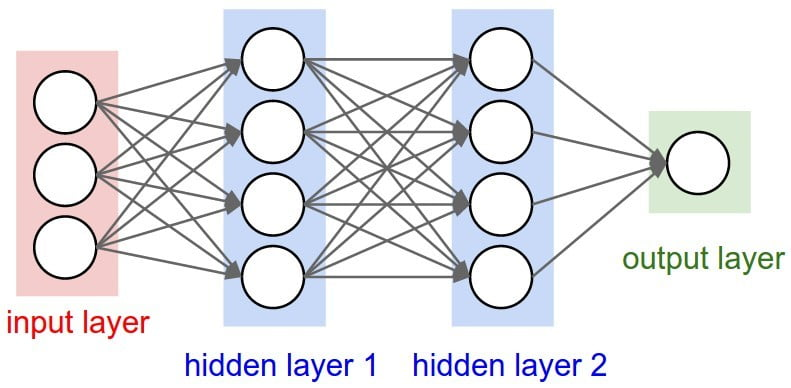
\includegraphics[width=12cm]{Images/ANN.jpg}
    \caption[Kiến trúc tổng quan của mô hình mạng thần kinh]
    {Kiến trúc tổng quan của mô hình mạng thần kinh - Stanford CS231n}
\end{figure}
\newpage
Trong một hệ thống mạng neural, các neural được phân làm 3 lớp chính khác nhau, bao gồm: Input Layer, Hidden Layer và Output Layer. Input Layer là lớp tiếp nhận các dữ liệu đầu vào và tiền xử lý dữ liệu. Lớp Hidden Layer thực hiện các bước rút trích, phân tích và tính toán các luồng dữ liệu nhận từ Input Layer, và có thể có một hoặc nhiều lớp khác nhau trong một hệ thống mạng neural. Còn lớp Ouput Layer có nhiệm vụ trả dữ liệu đầu ra của hệ thống, ví dụ như kết quả phân loại của một mô hình phân loại dữ liệu. Thông thường quá trình suy luận từ Input Layer cho đến tới Output Layer của mô hình mạng neural là quá trình lan truyền tiến (feedforward), tức là đầu vào các neural tại một lớp đều lấy từ kết quả các neural lớp trước đó mà không có quá trình suy luận ngược lại.

Ngoài ra, những kết nối giữa các neural còn được liên kết với một trọng số để thể hiện mức độ quan trọng của dữ liệu đầu vào trong quá trình xử lý thông tin cũng như quá trình chuyển đổi dữ liệu từ lớp này đến lớp khác. Thực chất, quá trình học của mạng neural chính là quá trình cân chỉnh trọng số liên kết giữa các kết nối cũng như từ dữ liệu đầu vào để đưa ra kết quả mong muốn.

\begin{figure}[htbp]
    \centering
    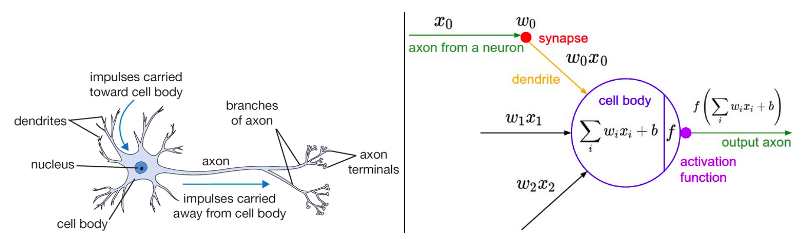
\includegraphics[width=13cm]{Images/neural.png}
    \caption[Cấu tạo của neural trong sinh học và trong mô hình ANN]
    {Cấu tạo của neural trong sinh học và trong mô hình ANN - Stanford CS231n}
\end{figure}

Cấu trúc của một neural bao gồm một hàm tổng (Summation Function) có vai trò tính toán các dữ liệu đầu vào cùng với trọng số có sẵn để đưa ra dữ liệu kết quả của neural đó. Kết quả này sẽ được đưa qua môt hàm kích hoạt (Activation Function) để quyết định xem neural đó có được phép hoạt động và cập nhập dữ liệu mới trên mô hình mạng hay không. Hàm kích hoạt giúp mô hình mạng neural có thể học hỏi được các mối quan hệ của dữ liệu hay thực hiện các tác vụ phức tạp khác, mà đa phần không phải là tuyến tính. Chính vì vậy, các hàm kích hoạt đều là hàm phi tuyến. Tùy thuộc vào hàm kích hoạt khác nhau sẽ có các công thức hàm khác nhau, ví dụ như hàm kích hoạt Sigmoid có công thức như sau:

\begin{equation*}
f_{S}(x) = \frac{1}{1 + e^{x}}\\
\end{equation*}

\chapter{MÔ HÌNH ĐỀ XUẤT}
\section{Mô hình}
\subsection{Mô hình nhận diện khuôn mặt}
Mô hình nhận diện khuôn mặt sử dụng giải thuật Facial Landmarks. Trong khi giải thuật gốc vẽ ra 81 điểm mốc bao quanh khuôn mặt, mô hình lược bỏ một số điểm mốc nhận diện mắt, mũi, môi, còn lại 30 điểm mốc bao quanh khuôn mặt như thể hiện ở hình~\ref{fig:Facial_Landmarks}.

\begin{figure}[ht]
    \centering
    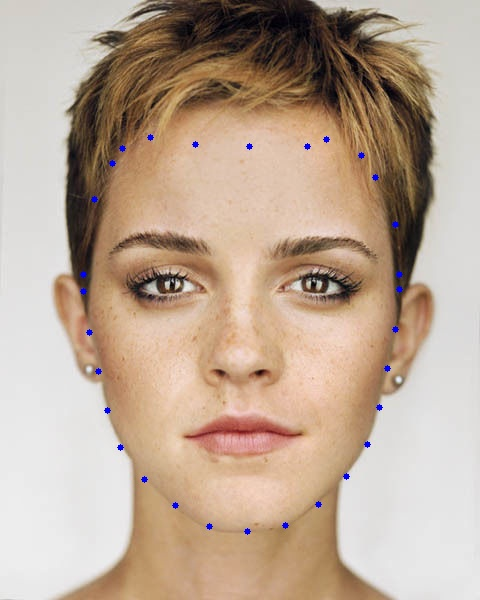
\includegraphics[width=5cm]{Images/Facial_Landmarks.jpg}
    \caption[Kết quả mô hình nhận diện khuôn mặt]
    {Kết quả mô hình nhận diện khuôn mặt với 30 điểm mốc}
    \label{fig:Facial_Landmarks}
\end{figure}
% \newpage
Căn cứ vào 30 điểm mốc bao quanh khuôn mặt, đề tài sử dụng công thức tính tỉ lệ khuôn mặt như sau:
\begin{equation}
R_{f} = \frac{N_{f}}{N}\\
\end{equation}
Với $N_{f}$ được tính bởi công thức~\ref{equa:polygon_area}, trong đó $(x_{n},y_{n})$ là tọa độ các điểm mốc được nhận dạng trên ảnh:
\begin{equation}
N_{f} = \sum_{1}^{n=30} \frac{\abs{(x_{1}y_{2} - y_{1}x_{2}) + (x_{2}y_{3} - y_{2}x_{3}) + ... + (x_{n}y_{1} - y_{n}x_{1})}}{2}\\
\label{equa:polygon_area}
\end{equation}
Trong đó:
\begin{itemize}[noitemsep]
\addtolength{\itemindent}{1.5cm}
    \item $R_{f}$: tỉ lệ khuôn mặt trên toàn bộ bức ảnh\\
    \item $N_{f}$: tổng diện tích khuôn mặt lọc bởi mô hình\\
    \item N: kích thước tấm ảnh
\end{itemize}
Tuy nhiên, mô hình nhận diện khuôn mặt vẫn có một số hạn chế khi thực nghiệm trên những khuôn mặt mờ hoặc xuất hiện không đầy đủ, thậm chí là những tấm ảnh chụp nghiêng. Những nhược điểm này sẽ được tìm cách khắc phục trong những công trình nghiên cứu sau.        
\chapter{THỰC NGHIỆM VÀ KẾT QUẢ}

Bảng~\ref{table:manually_category_2} và bảng~\ref{table:Result_1} thể hiện...

\begin{table}[htpt]
\begin{center}
\begin{tabular}{|c|c|c|c|}
\hline
 & Gán nhãn & Không gán nhãn  & \textbf{Tổng cộng}\\
\hline
Huấn luyện & 4000 & 0 & 4000\\
\hline
Tinh chỉnh & 1000 & 0 & 1000\\
\hline
Thực nghiệm & 500 & 40.000 & 40.500\\
\hline
\textbf{Tổng cộng} & \textbf{5500} & \textbf{40000} &  \textbf{45.500}\\
\hline
\end{tabular}
\caption{Caption 1}
\label{table:manually_category_2}
\end{center}
\end{table}

\begin{table}[htpt]
\begin{center}
\begin{tabular}{|c|c|c|c|c|c|c|}
\hline
\multirow{2}{*}{} & \multicolumn{3}{c|}{A} & \multicolumn{3}{c|}{B}\\
\cline{2-7}
& X & Y & Z & X & Y & Z \\
\hline
15 frame & 169 & 631 & 70 & 540 & 1460 & 76 \\
\hline
20 frame & 127 & 663 & 65 & 468 & 1532 & 73 \\
\hline
Bầu đa số & 88 & 712 & 60 & 291 & 1711 & 61 \\
\hline
\end{tabular}
\caption{Caption 2}
\label{table:Result_1}
\end{center}
\end{table}
\newpage
\chapter{KẾT LUẬN VÀ HƯỚNG PHÁT TRIỂN}

Như vậy, đề tài khóa luận đã đề ra 

% \input{Chapter/Conclusion.tex}
\begin{thebibliography}{99}               % trích dẫn
\addcontentsline{toc}{chapter}{{\bf Tài liệu tham khảo}\rm} 

\bibitem{cRCNN} Ross Girshick, Jeff Donahue, Trevor Darrell \& Jitendra Malik, \textit{Rich Feature Hierarchies for Accurate Object Detection and Semantic Segmentation}, Proceedings of the IEEE Computer Society Conference on Computer Vision and Pattern Recognition, 2013.

\bibitem{cFastRCNN} Ross Girshick, \textit{Fast R-CNN}, 2015.

\bibitem{cFasterRCNN} Shaoqing Ren, Kaiming He, Ross Girshick\& Jian Sun, \textit{Faster R-CNN: Towards Real-Time Object Detection with Region Proposal Networks}, IEEE Transactions on Pattern Analysis and Machine Intelligence, volume 39, 2015.

\bibitem{cMaskRCNN} Kaiming He, Georgia Gkioxari, Piotr Dollár and Ross B. Girshick. \textit{Mask R-CNN} 2017 IEEE International Conference on Computer Vision (ICCV), page 2980-2988, 2017.

\end{thebibliography}


\end{document}